% !TEX root = ../main.tex
%
\chapter{Conclusions} \label{sec:5}

The aim of this thesis work was to explore the feasibility of observing the \dst dibaryon in \pPb collisions 
at \sctev with the ALICE experiment.
The importance of this search lies in the fact that the measurement of the \ds signal would be the first
confirmation of the existence of non-trivial dibaryons.

The identification of the \ds is challenging because of the experimental conditions occurring in 
\pPb collisions. The choice of the \pPb data sample for this study was dictated by the necessity to have 
the maximum number of deuterons.
Indeed, if one does not take into account the \PbPb run, the 2016 \pPb data sample is characterized by the highest number of deuterons. 
The \PbPb data were not considered because of the high particle multiplicity produced in this colliding
system, which generates a huge combinatorial background that makes the \ds identification very difficult.
In pp collisions, instead, the deuteron production is lower than in \pPb by a factor of $\sim 3$, therefore
the analysis of the pp sample was excluded.

Nevertheless, the study of the background in \pPb collisions, performed in this thesis, showed that the
combinatorial background due to pions is crucial also in this colliding system and prevents the clear 
identification of the \ds decay. 
In addition, the expected wide shape of the \ds resonance contributes to make its identification even harder.
For these reasons, the resulting significance for the measurement of the \ds signal is as low as $\sim $ 0.25\ -- assuming that \ds
is produced according to the thermal model.

Upper limits were set for the production of the \ds dibaryon in \pPb collisions at \sctev, since there is
no evidence of its presence in the analysed data sample. The low significance of the measurement, however, 
leads to upper limits higher than the values predicted by the thermal model, thus not preventing to exclude that \ds is produced according to that model.

The detailed studies performed for this thesis work gave a clearer picture of the 
problems related to the search of the \ds dibaryon with the ALICE experiment. 
Furthermore, the analysis tools and methods developed for this work can be used in a future analysis.
Now it is clear that meaningful results can be achieved only by increasing the significance of the
measurement.
That increase can be achieved, basically, in two ways: by reducing the 
combinatorial background and by collecting a higher integrated luminosity.

A significant background reduction could be obtained searching the \ds in pp collisions.
Furthermore in pp collisions it is possible to improve the particle identification at low \pt
using the ITS detector, increasing the reconstruction efficiency.

\begin{figure} [htb]
    \centering
    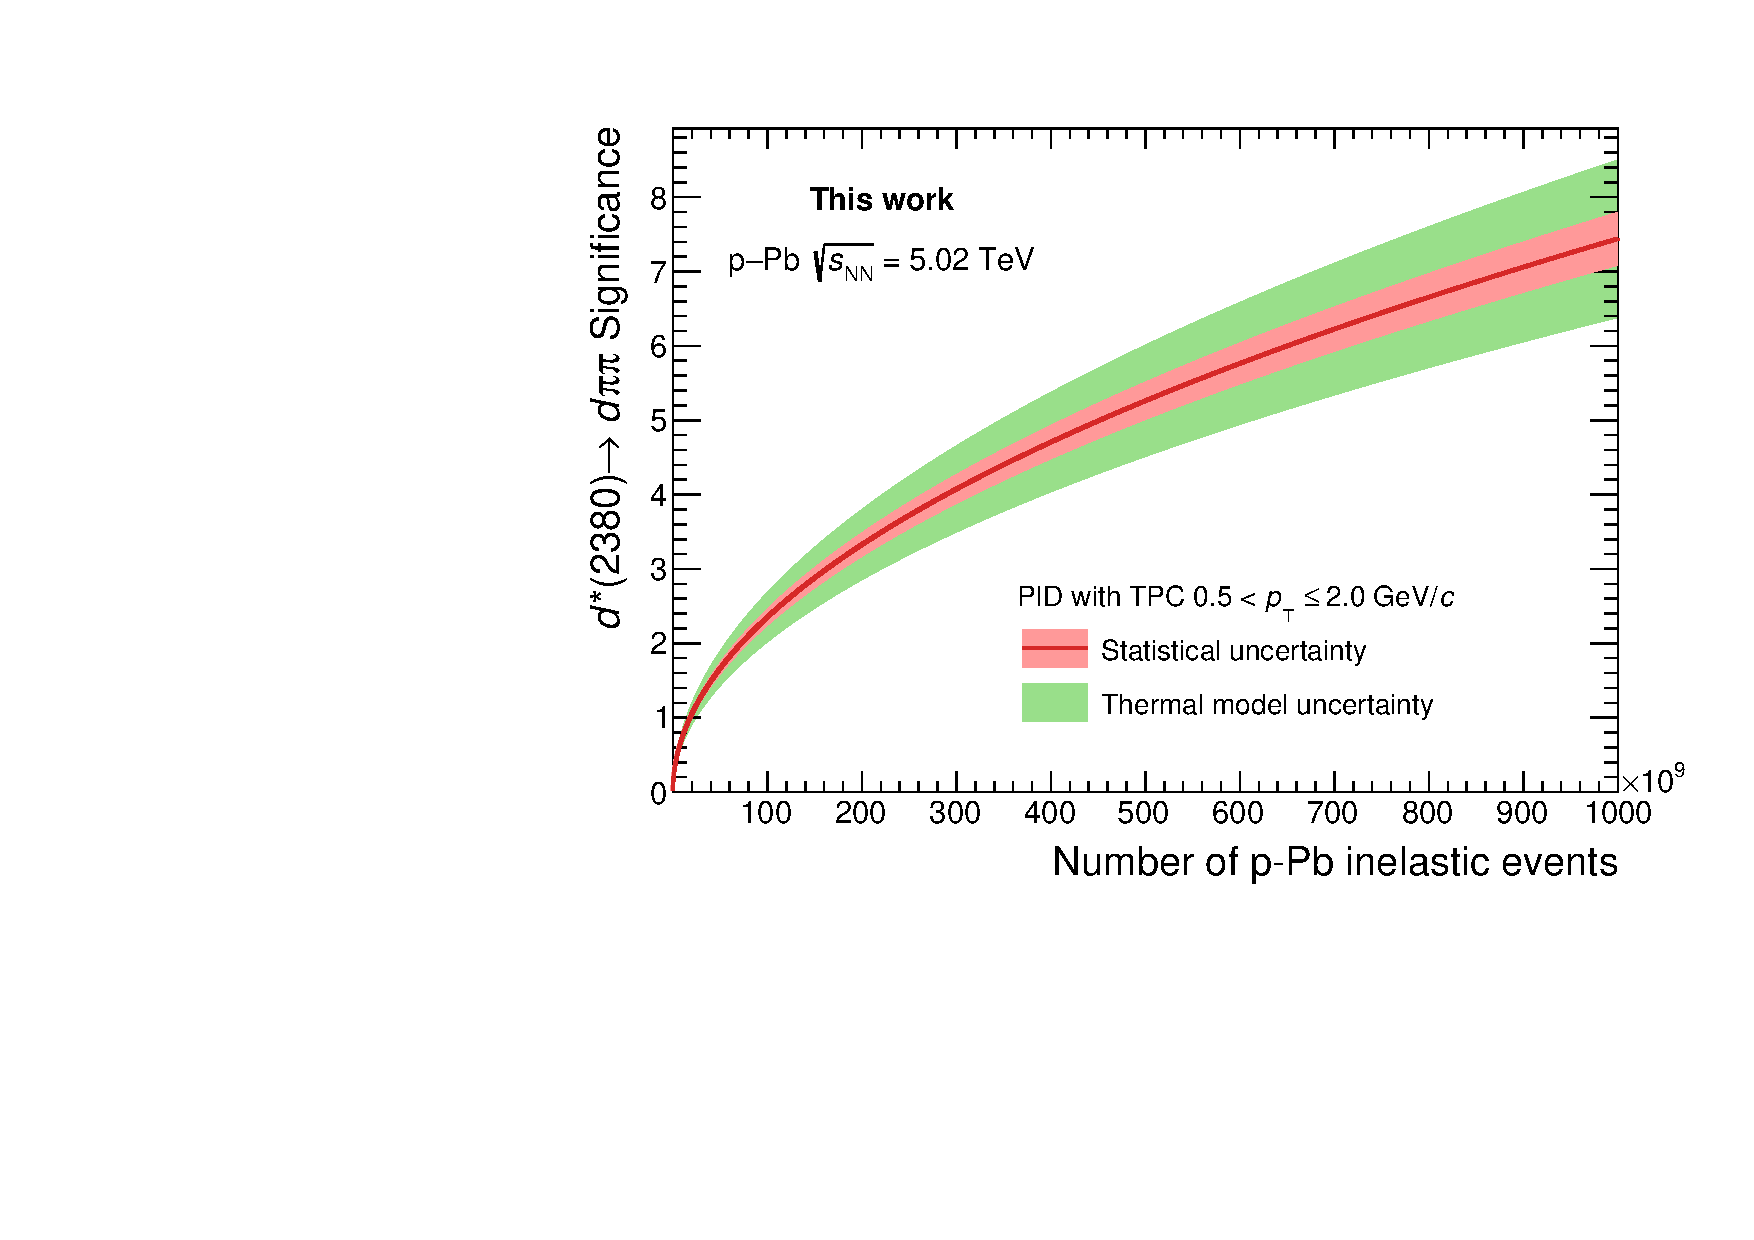
\includegraphics[width=0.85\textwidth]{gfx/sig_TPC}
    \caption{Significance as a function of the number of collected \pPb inelastic events using the TPC only particle identification configuration.}
	\label{fig:proj1}
\end{figure}

A final study was carried out to estimate the number of \pPb collisions needed to reach a
$5\;\sigma$ significance.
Figure~\ref{fig:proj1} shows that $\sim 5\times10^{11}$ events are needed to achieve this goal 
with the TPC configuration for particle identification (as described in Sec.~\ref{sec:ds_candidate}).
This number is far greater than the number of \pPb collisions available in the 2016 data sample
\ -- $5.5\times10^{8}$ minimum bias events.
This integrated luminosity is expected to be reached during the LHC Run 3 which will start in 2021.
Thanks to the tools and the analysis strategy developed during this thesis and to the larger data sample we will have at disposal, the search of the \ds dibaryon with the ALICE experiment will lead to significant results in the next years.
